\section{Synthèse non-ribosomique}
\label{bio_NRP}

\subsection{Introduction}
\label{intro_bio}

Afin de bien comprendre la voie de synthèse non ribosomique, commençons par quelques rappels rapides sur la synthèse des protéines classiques.
Dans la cellule, les protéines sont assemblées par un complexe moléculaire, appelé ribosome, qui lit les  les ARN messagers.
Ces ARN sont les vecteurs de l’information génétique et sont issus de la transcription d’un morceau d’ADN.
Ils sont traduits par triplets de nucléotides (appelés codons) en chaînes d’acides aminés.
Les 64 codons possibles ($4^3$ nucléotides) sont pour la plupart traduits en 20 acides aminés appelés acides aminés protéogéniques (car ils interviennent dans la synthèse classique de protéines).
Ces acides aminés sont tous composés d'un même squelette atomique autorisant deux liaisons et permettant ainsi la formation de chaînes peptidiques.
Sur le squelette est ancrée une chaîne latérale variant d'un acide aminé à l'autre, leur donnant leur spécificité (voir figure \ref{chaine_pep}).
Les deux liaisons qu'effectue le squelette sont supportées par un groupement amine ($NH_2$) et un groupement carboxyle ($C(=O)OH$).
Ces deux groupements se lient entre eux et créent ainsi une protéine linéaire.
Lorsque la chaîne n'est constitué que de quelques acides aminés (généralement moins de 25) on ne la nomme plus protéine mais peptide.

\begin{figure}[h!]
  \begin{center}
    \includegraphics[width=350px]{Figures/bio/Intro/chaine_pep.jpg}
    \caption{\label{chaine_pep}Présentation d'une chaîne peptidique.
    Chaque trait pointillé vertical sépare un acide aminé d'un autre et le trait horizontal sépare le squelette de la chaîne latérale des acides aminés.}
  \end{center}
\end{figure}

Une fois assemblée, une protéine se replie sur elle même et les caractéristiques structurelles et physico-chimiques qui en découlent lui donnent son activité.
Plus précisément, les propriétés des éléments en contact avec d'autres molécules détermineront l'activité de cette protéine.
Il est possible que ces surfaces soient à ``l'extérieur'' de la protéine ou à ``l'intérieur'' sous forme de poche.
Ces propriétés sont donc très dépendantes du repliement et des types des acides aminés exposés.



\subsection{Généralités sur les peptides non ribosomiques}
Les peptides non ribosomiques (Non Ribosomal Peptide -NRP-) sont des petits polymères synthétisés par certaines bactéries et certains champignons unicellulaires.
Tout comme les protéines classiques, les NRP sont des molécules résultant d'assemblages de briques de base.
Cependant, comme le nom l'indique, la voie de synthèse d'un NRP est différente de celle d'une protéine classique.
Cette voie de synthèse comporte une étape supplémentaire (voir figure \ref{global}).
Comme nous l'avons présenté en \ref{intro_bio}, lors d'une création classique de protéine, l'ADN est transcrit en ARN qui lui même est traduit en protéine.
Dans le cas d'une NRPS, la protéine produite n'est pas le produit final mais une \textit{enzyme modulaire} agissant seule ou en complexe afin d'assembler les NRP.
Ces complexes sont appelés des synthétases (Non Ribosomal Peptide Synthetase -NRPS-).

\begin{figure}[h!]
  \begin{center}
    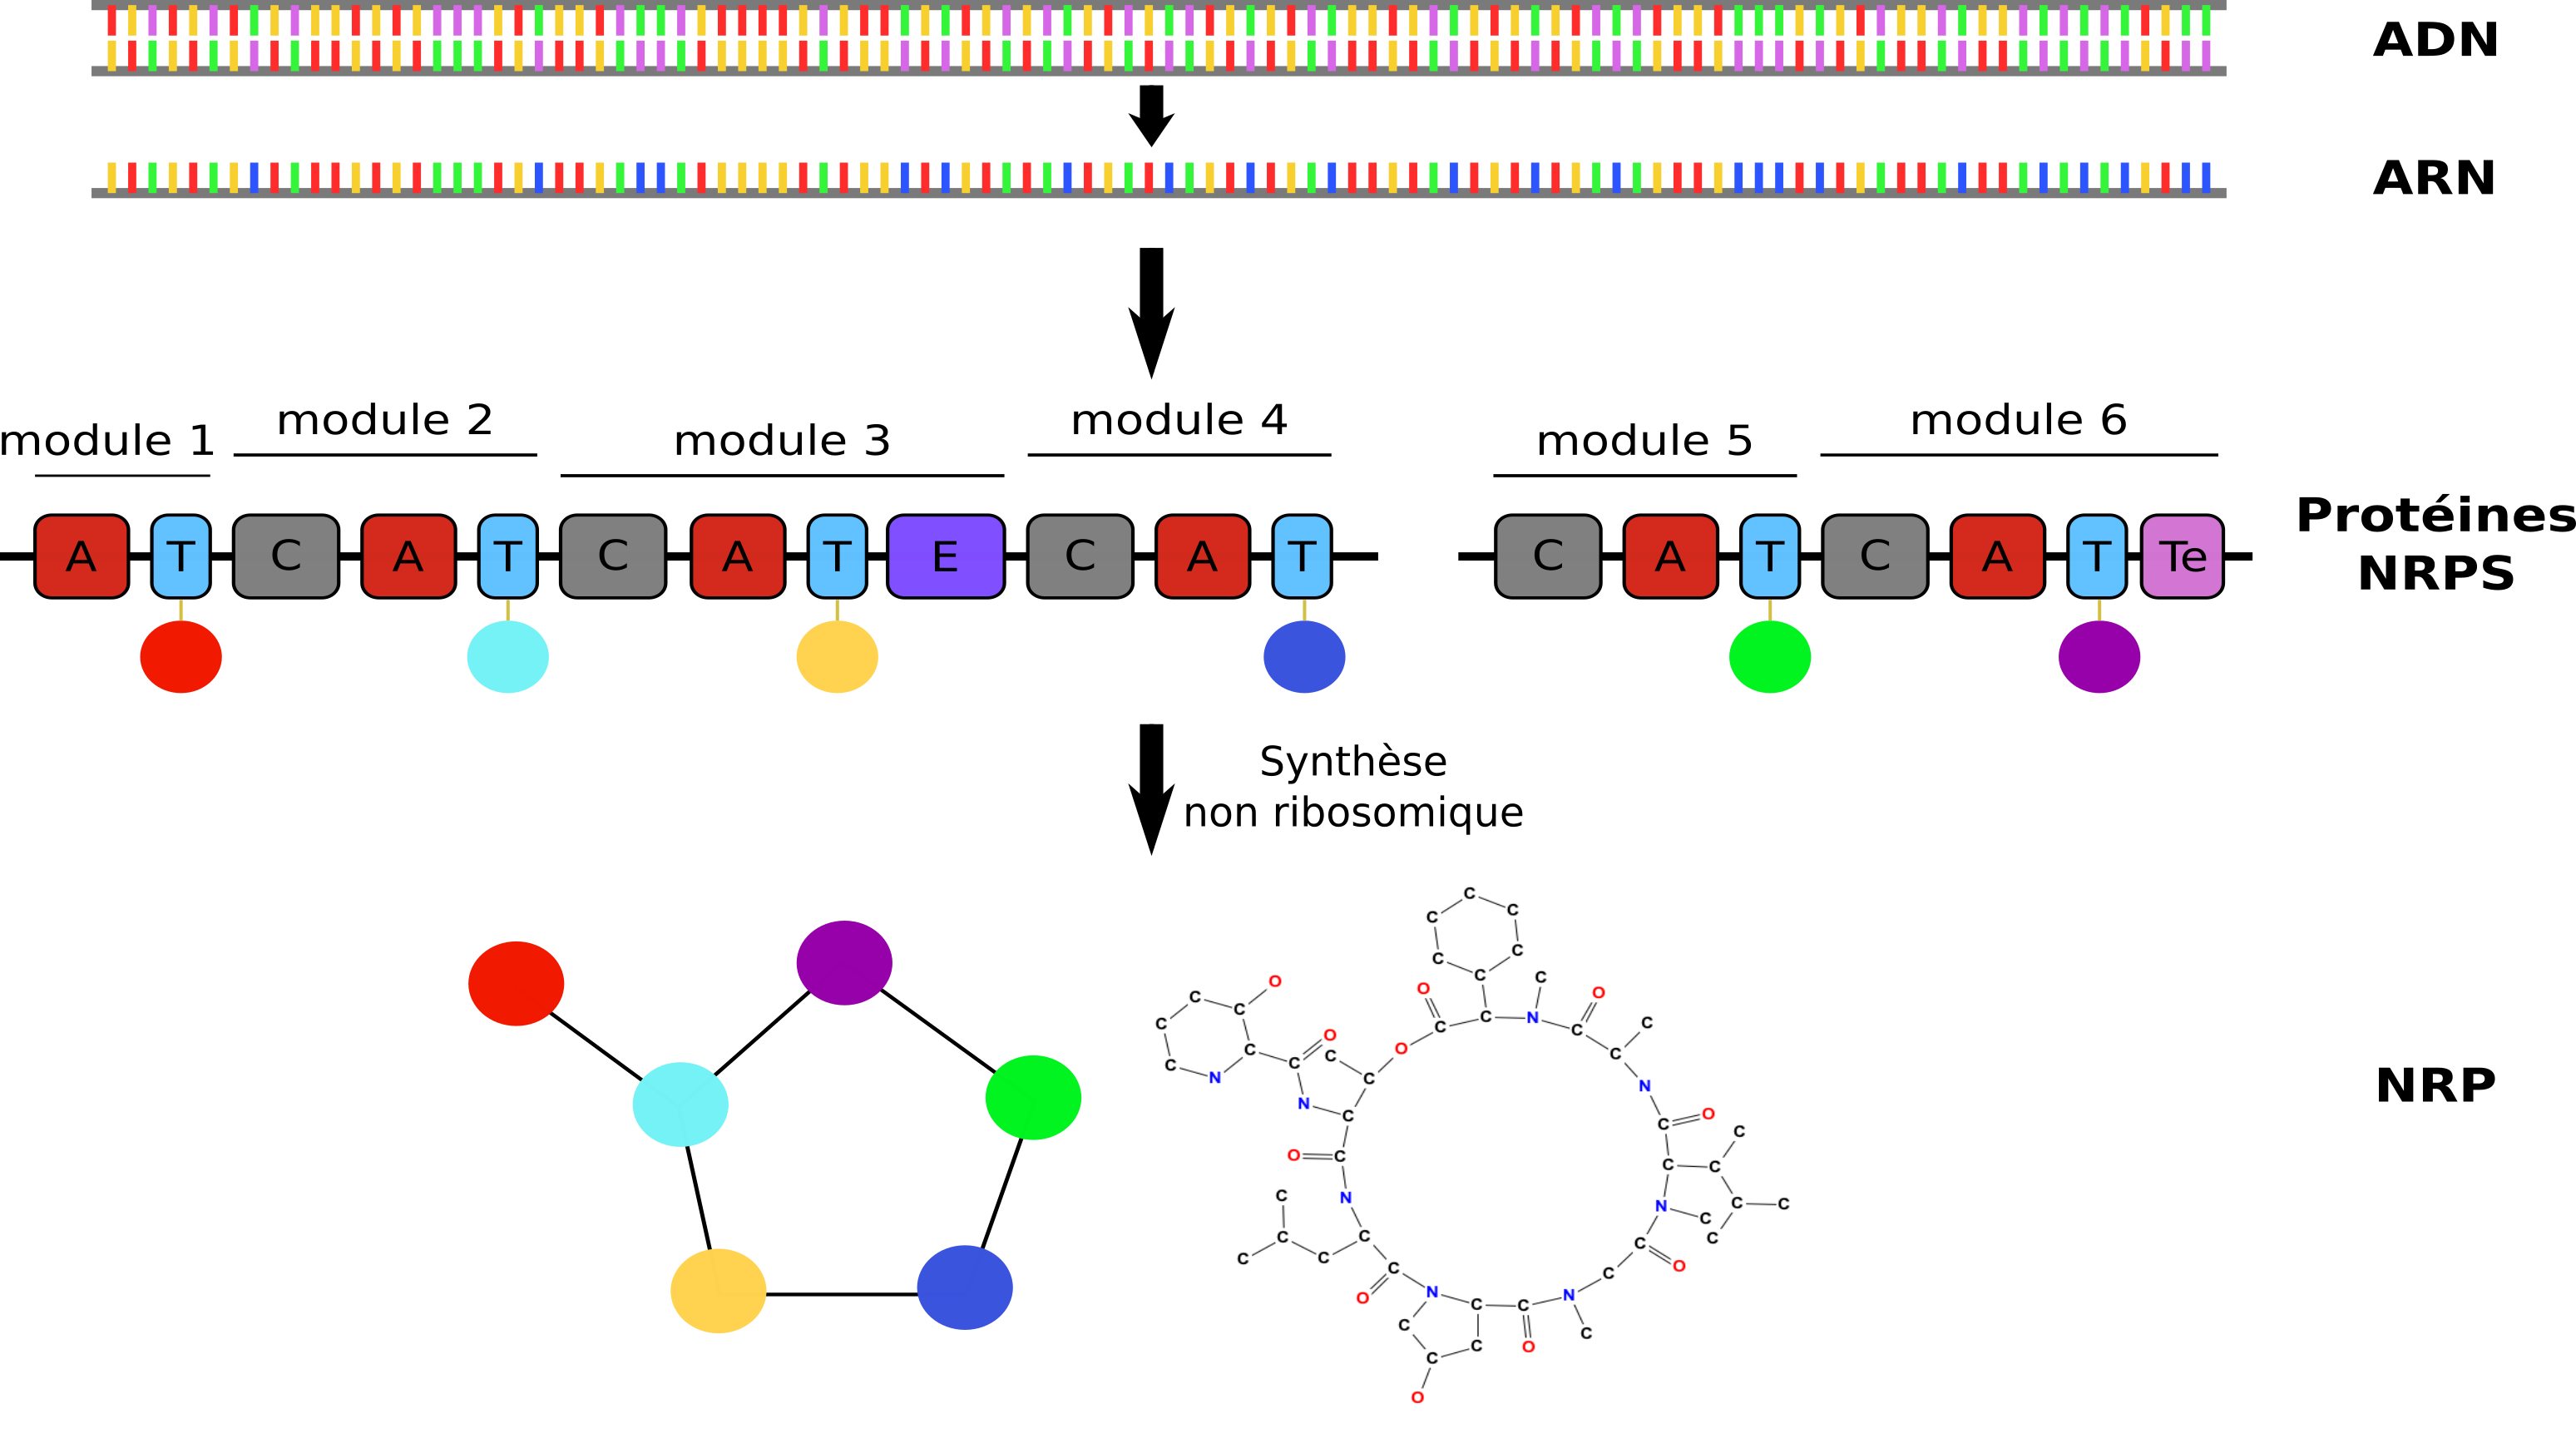
\includegraphics[width=450px]{Figures/bio/Intro/synthese.png}
    \caption{\label{global}Voie de synthèse non ribosomique~:
    groupés en cluster, les gènes codant les protéines NRPS sont transcrits puis traduits par le ribosome.
    Les domaines A de la NRPS capturent ensuite des monomères (billes de couleur ici) dans l'environnement afin de les assembler en peptide.
    Enfin, le NRP assemblé est relâché.
    }
  \end{center}
\end{figure}

\subsubsection{Les monomères}

\begin{figure}[h!]
  \begin{center}
    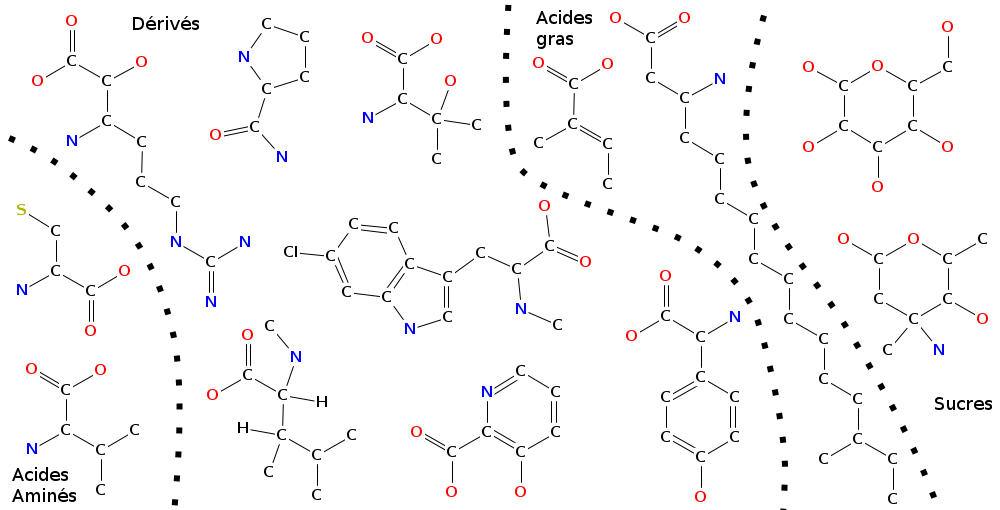
\includegraphics[width=450px]{Figures/bio/Intro/monos/monos.png}
    \caption{\label{monomers_example}Patchwork de monomères NRP.
    De gauche à droite : deux représentants des acides aminés classiques ; plusieurs dérivés d'acides aminés ; un acides gras ; deux sucres.}
  \end{center}
\end{figure}

Tandis que les protéines classiques sont majoritairement composées des 20 acides aminés standards, la synthèse non ribosomique incorpore plusieurs centaines de briques de base différentes.
Ces briques de base sont appelées {\em monomères}.
La base de données de référence des NRP compte pour le moment 533 monomères différents.
Les monomères peuvent provenir de différents groupes.
Parmi ces monomères, on compte les 20 acides aminés standards ainsi qu'un grand nombre de dérivés proches.
Après plusieurs modifications que nous détaillerons en section \ref{mono_modifs}, il est par exemple possible d'obtenir des monomères méthylés ou oxydés (voir figure \ref{monomers_example}).
On peut également citer les sucres et les acides gras comme faisant partie des monomères candidats à l'inclusion dans des NRP.


\subsubsection{Les structures peptidiques}

\begin{figure}[h!]
  \begin{center}
    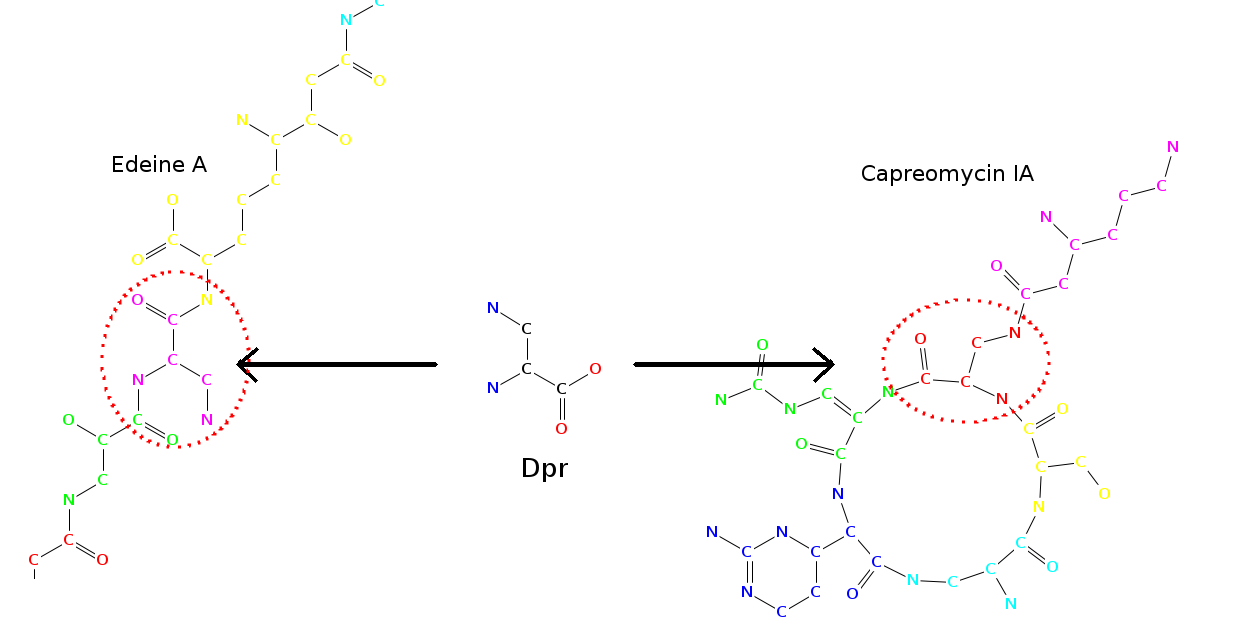
\includegraphics[width=400px]{Figures/bio/Intro/Dpr/2-3_liaisons.png}
    \caption{\label{DPR_incl}Deux exemples d'inclusion du monomère Dpr~:
    Au sein de l'Edeine A, seules les deux liaisons classiques du squelette peptidique sont effectuées entre le Dpr (en rose) et les autres monomères.
    Au sein de la Capreomycin IA, une troisième liaison est effectuée par le Dpr (en rouge) depuis son groupement amine ($NH_2$) de la chaîne latérale.}
  \end{center}
\end{figure}

Contrairement à la création des peptides classiques par le ribosome, les NRPS peuvent assembler les monomères au sein des NRP de manière non linéaire.
Certains monomères possèdent plus de deux groupements capables de réagir et former une liaison avec un autre monomère.
Ainsi sur l'exemple de la figure \ref{DPR_incl}, on peut constater que le monomère nommé Dpr (acide 2,3-diamonopropionique) possède un groupement amine supplémentaire à celui déjà présent dans le squelette des acides aminés classiques.
Ce groupement en bout de chaîne latérale autorise le Dpr à se lier 3 fois et ainsi casser la linéarité de la molécule assemblée.
Ces monomères permettent ainsi d'obtenir des structures à embranchements.


\subsubsection{Les liaisons inter-monomères}

Classiquement, les liaisons au sein de peptides se font par le rapprochement d'un groupement carboxyle d'un premier monomère vers le groupement amine d'un second.
Au sein des NRP, plusieurs autres types de liaisons viennent s'ajouter aux liaisons peptidiques.
Ceci augmente la diversité structurale des peptides.
La liaison peptidique classique reste tout de même la principale liaison effectuée entre monomères.
En dehors de celle-ci, nous pouvons lister trois différentes façons de lier les NRP.

Le premier type de liaison inclut un monomère contenant un atome de soufre.
Comme pour les protéines classiques, les monomères soufrés peuvent effectuer des ponts disulfure (liaison entre deux atomes de soufre en perdant deux atomes d'hydrogène).
Cependant, ce type de liaison n'est pas le seul impliquant un soufre.
Comme nous le verrons plus tard lors de la description des modules NRPS Cy (voir \ref{Cy}), l'atome de soufre peut également intervenir dans une cyclisation entre deux monomères en perdant son atome d'hydrogène de la même manière que lorsqu'il réalise un pont disulfure (voir figure \ref{Cy_link}).

\begin{figure}[h!]
  \begin{center}
    \includegraphics[width=400px]{Figures/bio/Intro/reactions/Cy.jpg}
    \caption{\label{Cy_link}Exemple de liaison effectuée par un domaine Cy}
  \end{center}
\end{figure}

Le second type de liaison implique au moins un monomère contenant un cycle aromatique (cycle imidazole ou benzène).
Dans les deux cas, c'est un atome d'hydrogène qui est arraché au cycle afin de pouvoir y lier un monomère.
Lors d'une liaison sur un cycle imidazole, c'est l'un des deux carbones voisins dans le cycle qui perdra un de ses hydrogènes au profit de la liaison avec l'autre monomère.
Dans le cas d'un benzène (Voir figure \ref{benzene}), c'est la présence d'un oxygène accroché au cycle qui permettra une affinité avec les carbones voisins.

\begin{figure}[h!]
  \begin{center}
    \includegraphics[width=400px]{Figures/bio/Intro/reactions/aro.jpg}
    \caption{\label{benzene}Exemple de liaison effectuée au sein d'un cycle benzène}
  \end{center}
\end{figure}

Enfin, le dernier type de liaison que nous allons décrire implique au moins un monomère de la catégorie des sucres (Glucose ou Arabinose par exemple).
Les sucres sont inclus sous leur forme cyclisée dans les NRP.
Suite à la liaison, un groupement OH a été perdu sur un carbone voisin de l'oxygène dans le cycle (voir figure \ref{ose}).
Face à eux, le monomère complémentaire ne perdra lui qu'un hydrogène pour former ainsi une molécule d'eau expulsée.

\begin{figure}[h!]
  \begin{center}
    \includegraphics[width=400px]{Figures/bio/Intro/reactions/ose.jpg}
    \caption{\label{ose}Exemple de liaison effectuée avec un sucre}
  \end{center}
\end{figure}

Cette diversité dans la façon de lier les monomères accompagnée du nombre de sites de liaisons candidats explique la diversité structurelle présente au sein des NRP.
La diversité du nombre de structures se voit aisément au sein des peptides représentés sur la figure \ref{peps_example}.

\begin{figure}[h!]
  \begin{center}
    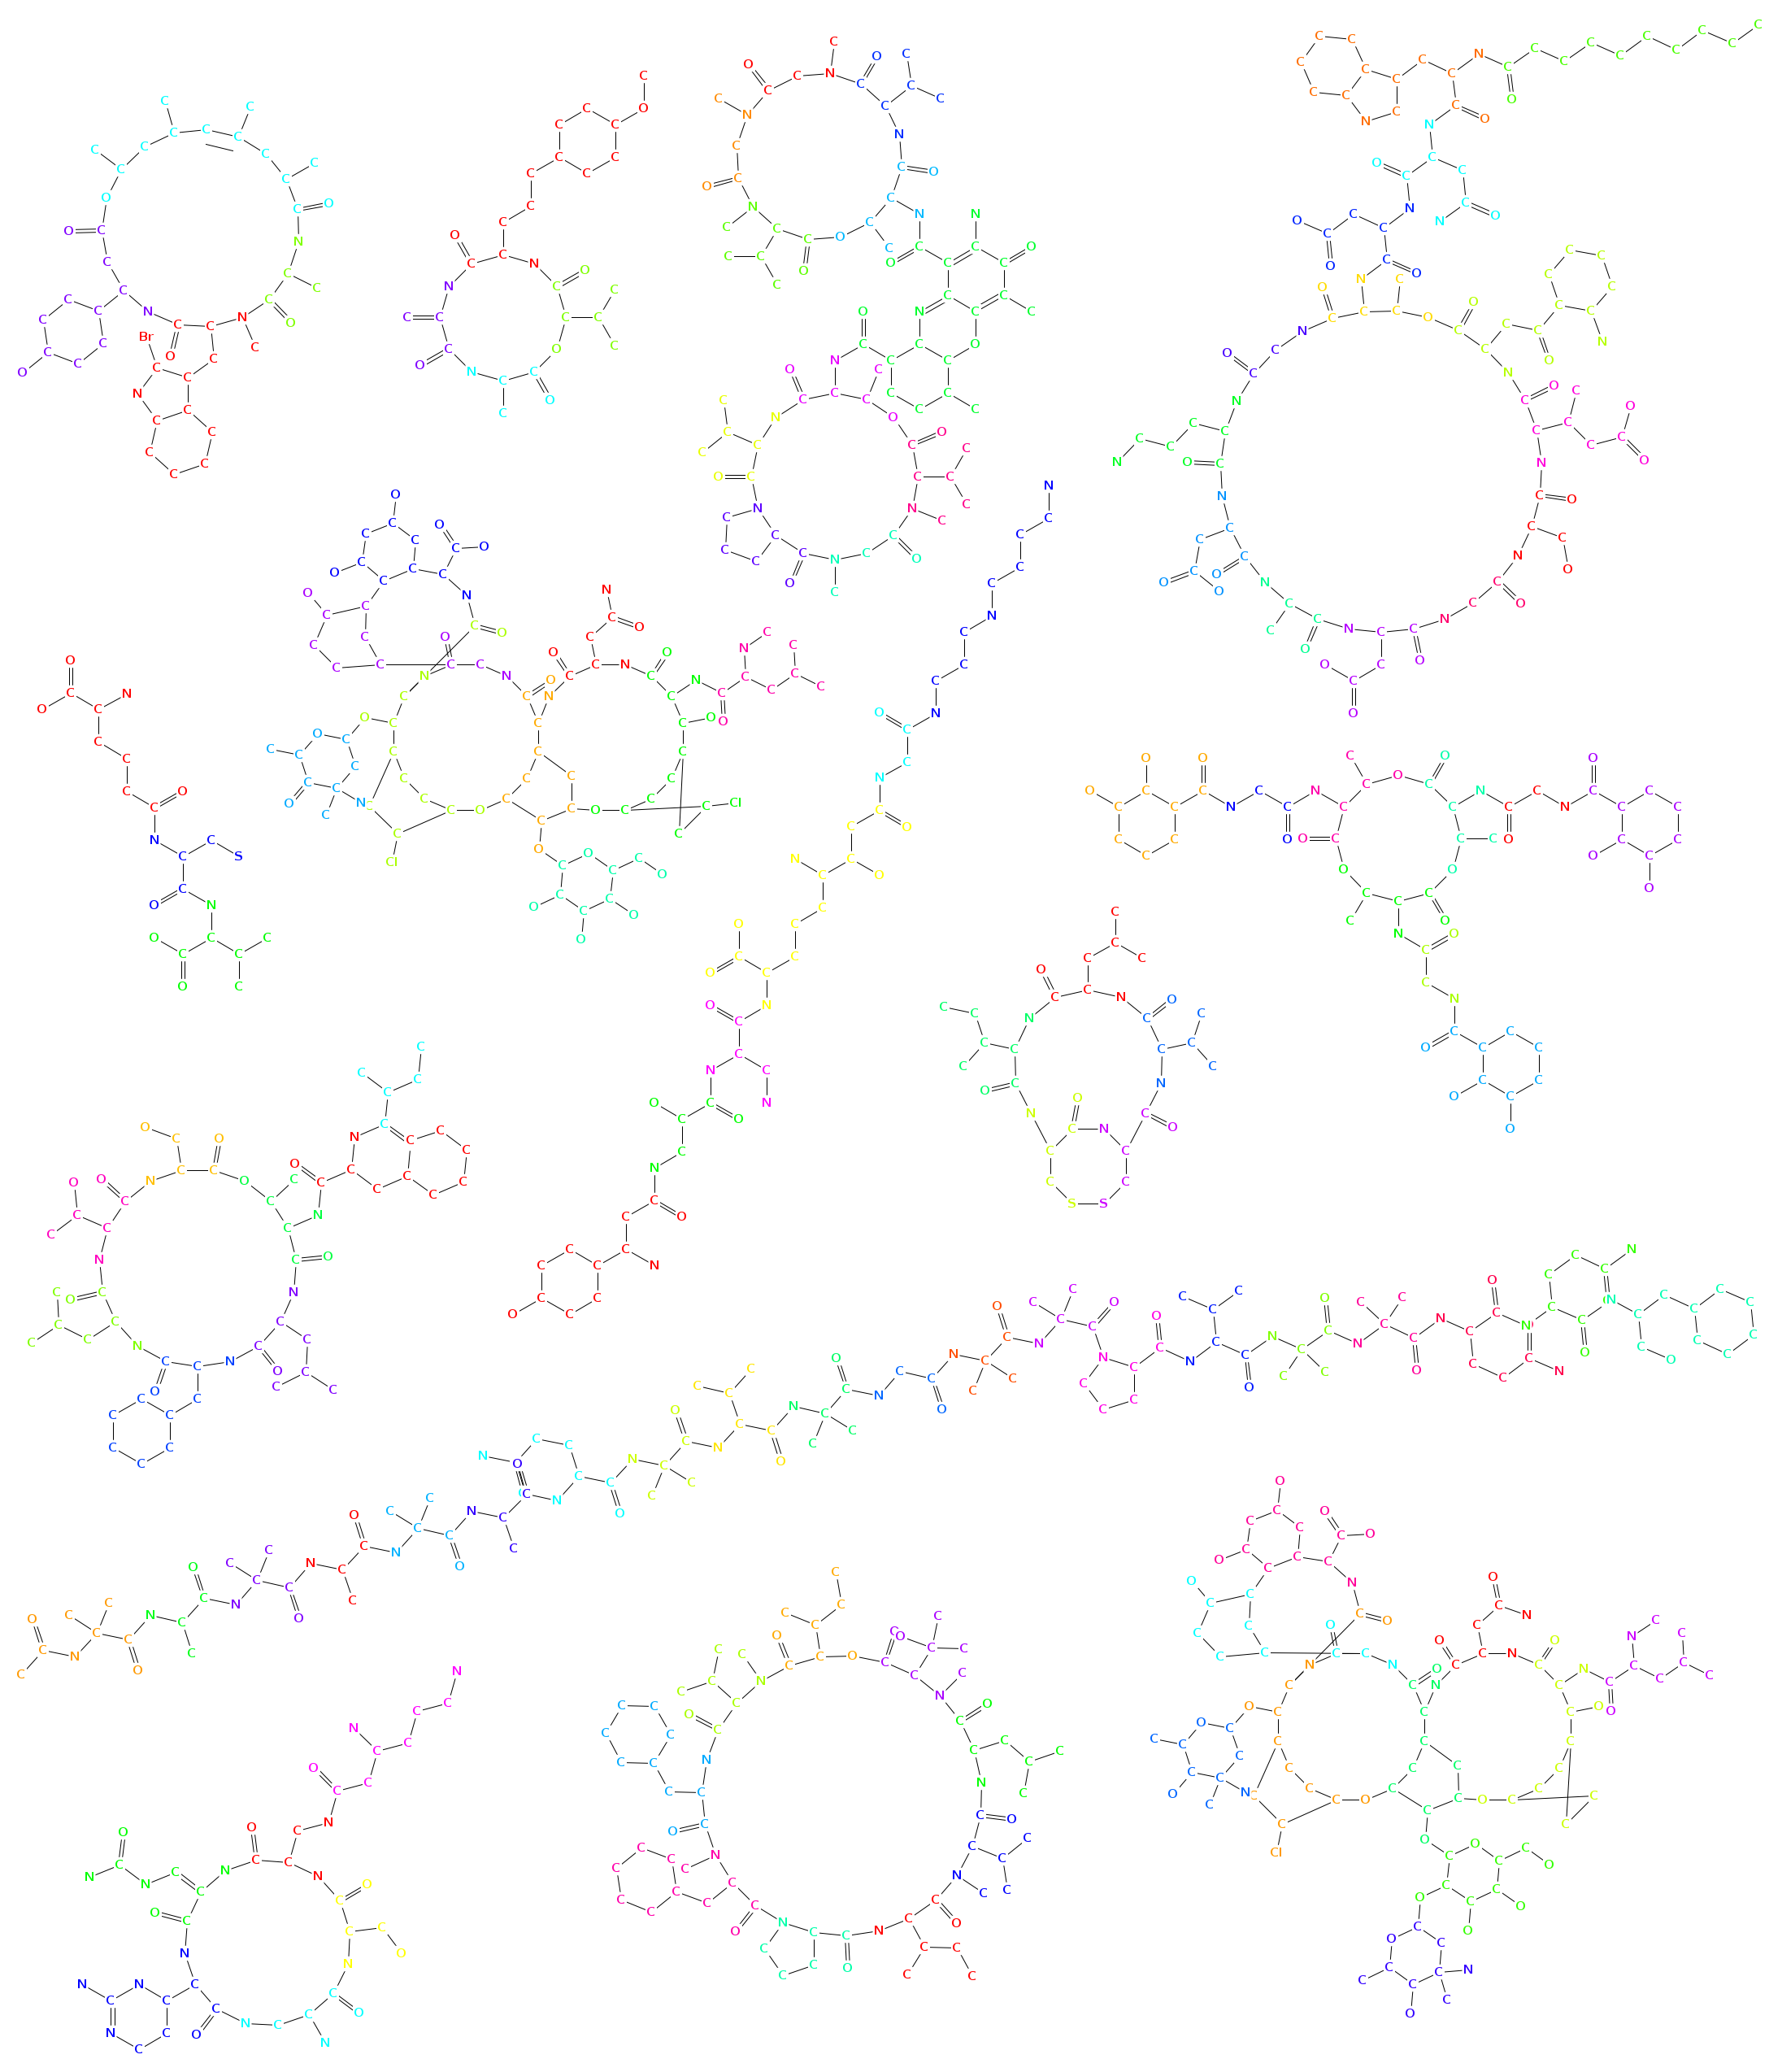
\includegraphics[width=450px]{Figures/bio/Intro/NRPs/peps.png}
    \caption{\label{peps_example}Patchwork de NRP}
  \end{center}
\end{figure}


\subsubsection{Les activités}

Les NRP présentent une grande diversité d'activités, souvent cruciales pour leurs producteurs.
Beaucoup de NRP recensés sont des antibiotiques comme par exemple, la célèbre molécule de pénicilline synthétisée à partir d'un précurseur NRP appelé ACV~\cite{queener_molecular_1990}.
La diversité d'activités peut être expliquée par les grandes variations de structures et de compositions par rapport aux peptides ribosomiques.
Les structures particulières et les divers monomères imposent aux NRP d'opter pour des repliements différents des protéines classiques.
Les contraintes structurelles permettent des repliements spécifiques qui ne sont pas possibles au sein des peptides classiques.
Les activités spécifiques aux NRP sont obtenues grâce à ces repliements et aux propriétés physico-chimiques des nombreux monomères.

Il est à noter qu'effectuer un assemblage non ribosomique est très consommateur en énergie pour l'organisme producteur.
Les complexes enzymatiques à créer sont énormes et les gènes portant leur information peuvent représenter plusieurs pourcents de l'ADN chromosomique.
De plus, contrairement au ribosome, une NRPS ne peut produire qu'un seul NRP (sauf quelques exceptions qui produisent des variants proches).
Cependant les avantages obtenus grâce aux activités des NRP semblent avoir préservé ces gènes au cours du temps.


\subsection{Généralités sur les synthétases}

Comme nous l'avons vu dans la courte introduction précédente, les synthétases qui assemblent les NRP sont des protéines issues d'une synthèse classique.
Chaque NRPS est un complexe enzymatique extrêmement grand, dont la taille est parfois comparable à celle d'un ribosome.
Cependant, contrairement à un ribosome, les NRPS sont spécialisées.
Une NRPS ne peut produire qu'un seul type de NRP.
Elles sont organisées en modules consécutifs qui capturent, modifient et intègrent un monomère au NRP~\cite{schwarzer_nonribosomal_2003,marahiel_modular_1997}.
Chacun de ces modules peut à son tour être subdivisé en domaines fonctionnels.
Généralement un module est constitué de 3 domaines principaux et éventuellement de domaines dits optionnels~\cite{finking_biosynthesis_2004}.
Un module standard est d'abord composé d'un domaine de condensation (C) effectuant la liaison du peptide déjà formé au monomère en cours d'incorporation, puis d'un module d'adénylation (A) permettant la capture du monomère à insérer et d'un module de thiolation (T) effectuant la fixation du monomère capturé et le transfert du NRP depuis le domaine C précédent au domaine C suivant.
Il se peut qu'un ou plusieurs domaines modifiant le monomère inclus, soient présents entre le domaine A et le domaine T.
Le tout premier module d'une NRPS est différent du fait qu'il n'y a aucun monomère à lier auparavant.
Il est l'une des exceptions à la règle de succession des modules C, A puis T.

\begin{figure}[h!]
  \begin{center}
    \includegraphics[width=480px]{Figures/bio/Intro/hc-toxin.png}
    \caption{\label{mibig_hc}Modules NRPS pour la création du peptide HC-Toxin.
    Image issue du site web MiBIG.Les ovales bleus ciels représentent les domaines T.}
  \end{center}
\end{figure}

Prenons pour exemple le NRP appelé HC-toxin~\cite{_mibig:_????}.
Le HC-toxin est un peptide non ribosomique composé de 4 monomères.
D'après la base de données MiBig~\cite{medema_minimum_2015} couplée à celle du NCBI~\cite{ncbi_resource_coordinators_database_2013}, la synthétase permettant sa création est composée de 5218 acides aminés.
Cette enzyme peut être séparée en 4 modules, incluant chacun un monomère.
Chacun des modules est également subdivisé en domaines.
Le découpage pour ce NRP est représenté sur la figure~\ref{mibig_hc}.
Aux 4 modules correspondent 4 domaines A, 4 domaines T et 4 domaines C.
On peut également voir un domaine d'épimérisation (modification de l'acide aminé inclus) présent en fin de premier domaine.
Dans le cas de cette NRPS, le domaine C en fin d'enzyme effectue la cyclisation du peptide.

\subsection{Les domaines principaux}

\subsubsection{Le domaine d'Adénylation (domaine A)}

Le domaine d'adénylation (A) réalise la capture dans l'environnement d'un type de monomère donné.
Il porte ainsi la spécificité du module dans lequel il se trouve.
La séquence d'acides aminés de ce type de domaine varie fortement d'un domaine A à l'autre et seuls 16\% de séquence du domaine sont conservées (sur environ 200 acides aminés codant un domaine)~\cite{stachelhaus_specificity-conferring_1999}.
Bien que seuls quelques domaines A aient été caractérisés, on suppose qu'il en existe un grand nombre (potentiellement plusieurs centaines) puisque
plusieurs centaines de monomères différents sont inclus par ces domaines.

Une fois le repliement de la synthétase effectué, les domaines A possèdent une cavité interne effectuant la reconnaissance et l'accueil d'une molécule.
Les acides aminés de la synthétase formant cette cavité vont ``sélectionner'' le monomère à capturer dans l'environnement.
La taille de la cavité ainsi que les propriétés physico-chimiques de ces acides aminés en contact permettent une affinité forte avec un unique monomère.
Il arrive parfois que le domaine ne soit pas spécifique à un seul monomère mais plutôt à un petit nombre de monomères très proches les uns des autres.
Cependant, ce cas reste rare et, dans la majorité des cas, une NRPS ne crée qu'un seul NRP.

En 1999, Stachelhaus \textit{et al}. publient un article analysant la structure de nombreux domaines A~\cite{stachelhaus_specificity-conferring_1999}.
Ils alignent un grand nombre de domaines A pour en extraire les zones conservées et les zones spécifiques au monomère à capturer.
Il apparaît tout d'abord que peu d'acides aminés sont conservés d'une structure à l'autre.
Cependant ces acides aminés permettent de définir le ``squelette'' d'un domaine A.
Ces alignements permettent également d'identifier une dizaine d'acides aminés qui paraissent spécifiques au monomère inclus.
À partir de ces acides aminés spécifiques, les auteurs déterminent un codage pour chaque monomère qui deviendra le codage de référence.
Ce codage est aujourd'hui appelé \textit{code de Stachelhaus} et permet de mettre en relation une séquence d'un domaine A et le monomère spécifiquement recruté.


\subsubsection{Le domaine de Thiolation (domaine T)}

Le rôle du domaine T est d'assurer le transport du peptide en cours d'élongation au sein du module~\cite{stachelhaus_biochemical_1996,calcott_portability_2015}.
Ce domaine est également souvent appelé ``Peptidyl Carrier domain''.
Chaque domaine T possède un groupement \textit{4’-phosphopantetheinyl} incluant un ``bras flexible'' qui agrippe et déplace les monomères.
Dans un premier temps, ce bras se plie vers le domaine A voisin pour se lier de manière covalente au monomère.
Dans un second temps, le monomère est mené au site de condensation afin d'être inséré en bout du NRP.
Enfin, le bras se plie dans la direction du domaine de condensation suivant afin de lier le NRP au monomère suivant.
Durant cette étape, le peptide est libéré du domaine T courant pour être laissé à la charge du domaine T suivant.

\begin{figure}[h!]
  \begin{center}
    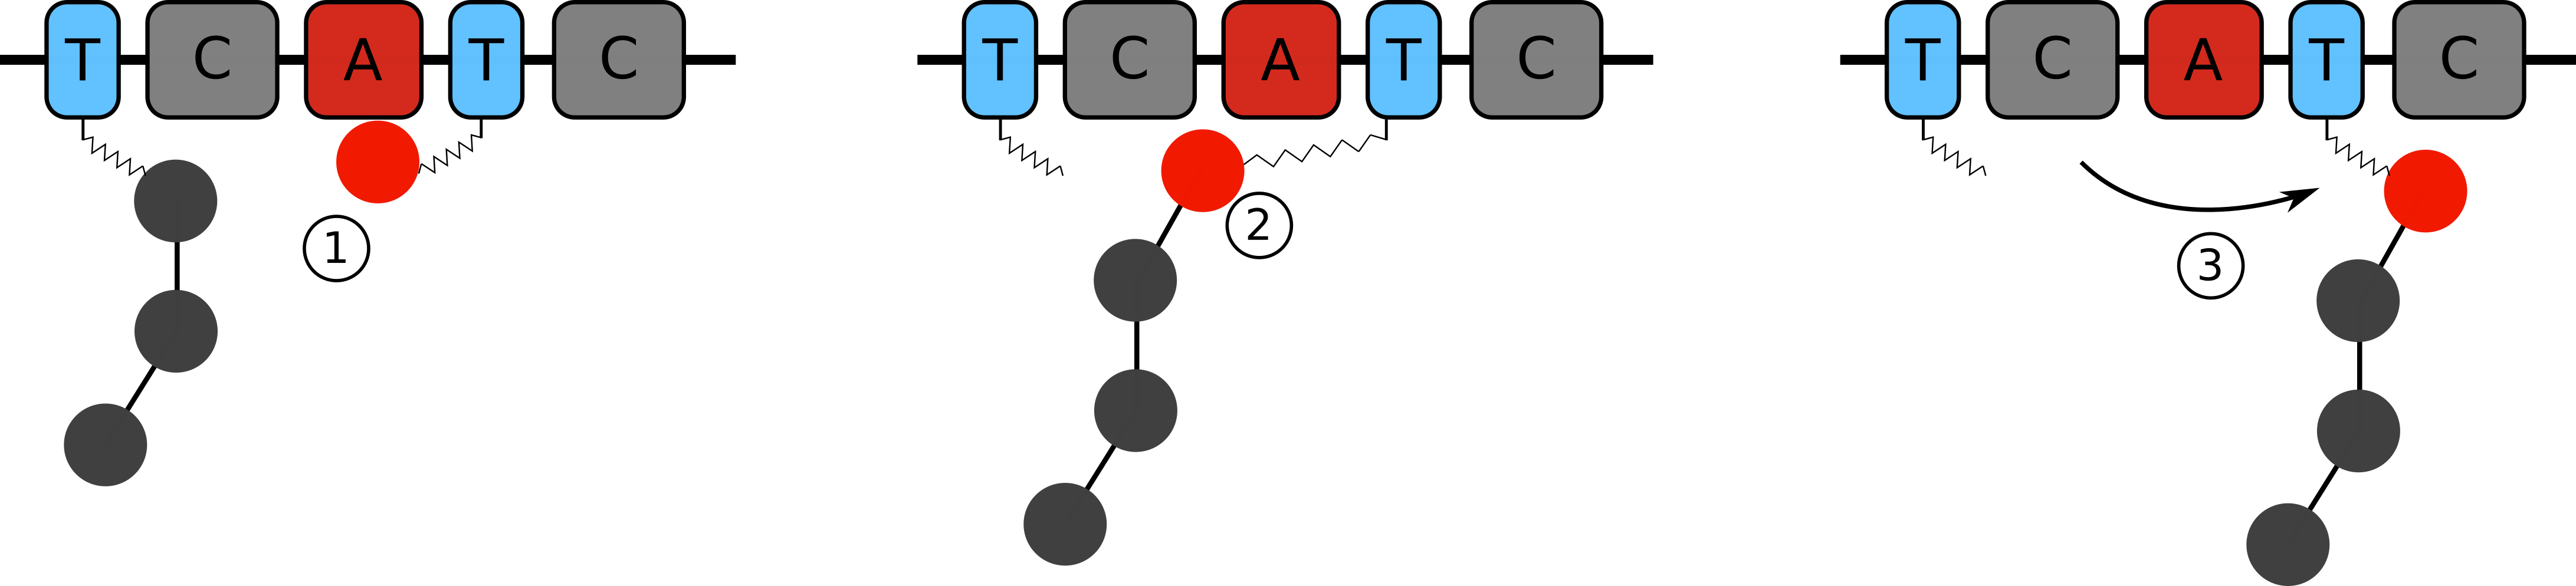
\includegraphics[width=450px]{Figures/bio/Intro/T-domain.png}
    \caption{\label{T_domain}Rôle du domaine T au sein d'une NRPS.
    1~- Liaison entre le monomère capturé par le domaine A et le bras du module T.
    2~- Liaison entre le monomère et la chaîne peptidique en cours d'élongation.
    3~- Déplacement du peptide vers le domaine C suivant}
  \end{center}
\end{figure}

\subsubsection{Le domaine de Condensation (domaine C)}

Le domaine C est par convention considéré comme le premier domaine de chaque module~\cite{stachelhaus_peptide_1998}.
C'est un domaine qui lie le morceau de peptide assemblé par les modules précédents avec le monomère capturé par le domaine A du module courant.
Bien que sa fonction principale reste omniprésente, il existe plusieurs variants~\cite{rausch_phylogenetic_2007} de ce domaine que nous allons décrire par la suite.

\textbf{Les domaines \textsuperscript{L}C\textsubscript{L} et \textsuperscript{D}C\textsubscript{L}}
Les acides aminés capturés par les domaines A existent dans deux configurations différentes dites configurations L (Levogyre) et D (Dextrogyre).
Ces configurations seront un peu plus détaillées en section \ref{epimeri}.
Il existe deux domaines C différents pour lier ces molécules.
Le plus standard, lie deux monomères de type L. Le domaine est alors appelé domaine \textsuperscript{L}C\textsubscript{L}.
Le second lui, lie un monomère D à un L, il est alors appelé domaine \textsuperscript{D}C\textsubscript{L}.
Ces domaines sont juste deux spécialisations du modèle décrit ci-dessus.

\textbf{Les domaines C starter (Cs) et C terminal (Ct)}
Comme leurs noms l'indiquent, ces domaines sont positionnés aux extrémités des synthétases.
Ils ne sont donc pas entourés de deux modules différents mais sont inclus respectivement dans le premier ou dernier module.
Il ne peuvent donc faire la liaison entre deux monomères fixés sur deux bras de domaines T.

Le domaine Cs capture et lie directement un monomère de l'environnement afin de débuter le peptide.
Cela permet d'inclure par exemple les acides gras car ils ne sont pas reconnus par les domaines A.
Ces modules capturent toujours le même type de monomères mais on ne sait actuellement pas exactement comment cette spécificité est encodée dans l'enzyme.

Le domaine Ct est un domaine de cyclisation uniquement présent chez les champignons.
Dans certains peptides, ce domaine effectue une liaison entre le premier et le dernier monomère du peptide en cours de formation, créant ainsi un cycle\cite{gao_cyclization_2012}.

\textbf{Le domaine Cy}
\label{Cy}
Cette dernière variation du domaine C lie deux monomères voisins en effectuant deux liaisons qui forment un cycle local (voir figure \ref{domaine_Cy}).
Cette liaison est toujours effectuée entre un monomère possédant un atome de soufre près d'un groupement amine (la Cystéine et certains de ses dérivés) et un monomère avec un groupement carboxyle.

\begin{figure}[h!]
  \begin{center}
    \includegraphics[width=300px]{Figures/bio/Intro/domainCy_bacitracine.png}
    \caption{\label{domaine_Cy}Cyclisation entre deux monomères par un domaine Cy}
  \end{center}
\end{figure}


\subsubsection{Le domaine de Thioestérase}

Le domaine Te fait partie du module de terminaison.
Il est le dernier domaine de ce module et vient succéder au domaine T ou aux domaines optionnels présents après le T.
C'est un domaine de terminaison qui permet le décrochage et parfois la cyclisation du peptide complètement formé~\cite{trauger_peptide_2000,kohli_thioesterase_2002}.
Ce domaine de libération n'est pas toujours présent et sa fonction est parfois assumée par d'autres domaines comme le domaine Ct.


\subsection{Les domaines de modification des monomères}

\label{mono_modifs}

Nous allons à présent décrire quelques domaines optionnels modifiant un monomère capturé par un domaine A au cours de la synthèse peptidique.
Ces transformations permettent aux organismes d'obtenir des configurations monomériques peu fréquentes dans leur environnement.


\subsubsection{La fonction d'épimérisation (domaines E et C/E)}
\label{epimeri}

Lors de la description des domaines \textsuperscript{L}C\textsubscript{L} et \textsuperscript{D}C\textsubscript{L}, nous avons rapidement évoqué la possibilité pour un monomère d'être dans deux conformations différentes tout en possédant pour autant la même composition et structure atomique.
Ces deux conformations sont symétriques l'une de l'autre.
Elles sont appelées Levogyre (L) et Dextrogyre (D).

\begin{figure}[h!]
  \begin{center}
    \includegraphics[width=400px]{Figures/bio/Intro/domaineE-bacitracine.png}
    \caption{\label{domaine_E}Épimérisation d'un monomère par un domaine E}
  \end{center}
\end{figure}

Alors que la majorité de la vie est ``gauchère'' (ne contient que des acides aminés L), les NRPS autorisent l'inclusion de monomères sous forme D par la capture d'un monomère L qui est ensuite transformé dans sa configuration D.
Les domaines responsables de ces transformations sont appelés domaines d'\textit{épimérisation}~\cite{calcott_portability_2015}.
Une fois le monomère L lié au reste du peptide par le domaine C, il est emmené auprès du domaine E qui va changer son orientation.
Le fait que cette transformation soit postérieure à la fixation sur le reste du peptide explique l'absence de domaines \textsuperscript{D}C\textsubscript{D} (Les monomères de droite seront toujours présentés au domaine C avant transformation).
Il arrive parfois que cette transformation du monomère ne soit pas portée par un domaine E mais directement incluse dans le domaine C précédent.
Ce domaine est alors appelé domaine C/E et assure les deux fonctionnalités~\cite{yin_enduracidin_2006,balibar_generation_2005}.
Ceci semble spécifique à quelques genres de bactéries.


\subsubsection{Domaine de N-méthylation (NM)}

De la même manière que le domaine E, le domaine NM agit à la suite de la liaison du monomère actuel à la chaîne peptidique précédemment assemblée.
Ce domaine ajoute un méthyle ($CH_{3}$) sur le groupement amine du monomère courant.

\begin{figure}[h!]
  \begin{center}
    \includegraphics[width=300px]{Figures/bio/Intro/domaineNMe-cyclosporine.png}
    \caption{\label{domaine_NMe}Méthylation d'un monomère par un domaine NM}
  \end{center}
\end{figure}

\subsubsection{Domaine de formylation}
% http://archiv.ub.uni-marburg.de/diss/z2008/0068/pdf/dgs.pdf

Ce domaine n'existe a priori que pour les modules d'initiation.
Il permet la formylation (ajout d'un groupe C(=O)H) sur le groupement amine du premier monomère~\cite{schonafinger_amide_2007}.

\begin{figure}[h!]
  \begin{center}
    \includegraphics[width=300px]{Figures/bio/Intro/domaineF-gramicidine.png}
    \caption{\label{domaine_F}Formylation d'un monomère par un domaine F}
  \end{center}
\end{figure}


\subsection{Incorporations extra-NRPS}

Depuis le début de cette partie, nous parlons de synthèse non ribosomique.
Cependant, il arrive que le produit délivré par la synthétase et le produit final trouvé dans l'environnement de la cellule ne soient pas les mêmes.
Lorsque cette différence est constatée, c'est que le peptide a subi une transformation entre la fin de sa synthèse non ribosomique et le moment où il est effectivement en activité.
Toutes les modifications ponctuelles sont effectuées par des \textit{enzymes de décoration} (voir section \ref{sucres}).
Parfois, il arrive que ce soit une partie complète de la molécule qui ne soit pas NRP.
Il existe également des molécules très proches des NRP appelés polyketides qui peuvent venir s'hybrider avec des NRP (voir section \ref{PKS_p}).
Dans cette partie, nous allons aborder ces deux types de modification/ajout d'un NRP.


\subsubsection{Les enzymes de décoration}

\label{sucres}

Les clusters de gènes de NRPS ne sont pas uniquement constitués des gènes d'enzymes NRPS.
De nombreux gènes accessoires sont également présents, généralement inclus dans le cluster.
Parmi ceux-ci, certains gènes servent à modifier les NRP déjà relâchés par la NRPS.
La \textit{vancomycine} est un très bon exemple de peptide subissant des modifications enzymatiques post-synthèse.

\begin{figure}[h!]
  \begin{center}
    \includegraphics[width=300px]{Figures/bio/Intro/vanco.png}
    \caption{\label{vanco}Modifications post-synthèse NRP pour la vancomycine}
  \end{center}
\end{figure}

Sur la figure \ref{vanco}, les deux structures entourées en vert se démarquent par rapport au reste de la molécule.
Ce sont deux sucres qui ont été ajoutés après la synthèse (une \textit{vancosamine} et un \textit{D-glucose}).
Les sucres sont des monomères qui ne peuvent pas être capturés par des domaines A.
Ce sont des gènes extérieurs à la NRPS mais faisant partie du cluster, qui sont dédiés à leur capture, transformation et liaison avec le NRP.
Ce phénomène d'ajout de sucre est appelé \textit{glycosylation}.
Comme le suggère A. van Wageningen~\cite{van_wageningen_sequencing_1998}, trois enzymes entrent en action pour incorporer la vancosamine.
La vancosamine n'étant pas naturellement présente dans l'environnement de l'organisme producteur, l'une des enzymes est dédiée à la création de ce sucre à partir du \textit{NDP-4-keto-6-deoxyglucose}.

La vancomycine possède également deux atomes de chlore.
Ces deux atomes sont inhabituels pour des NRP et ne sont pas initialement présents au sein de leurs monomères de base.
Il n'existe pas non plus de domaine NRPS capable d'inclure ces atomes.
A. van Wageningen dans l'article précédemment cité, montre également que deux gènes d'enzymes présents dans le cluster de la NRPS sont responsables de ces incorporations.
Ce type d'enzyme est appelé enzyme d'\textit{halogénation} car il est capable d'inclure un atome halogène (fluor, chlore, brome, iode)

Pour résumer, les enzymes de décoration post-synthèse sont capables d'effectuer 3 tâches que nous avons découvertes sur l'exemple de la vancomycine :
\begin{itemize}
  \item La synthèse de monomères en modifiant des composants de l'environnement (par exemple, création de vancosamine)
  \item La création de liaisons entre monomères de l'environnement et NRP (par exemple, les sucres de la vancomycine)
  \item La modification de monomères déjà inclus dans le NRP (halogénation par exemple)
\end{itemize}

Toutes ces enzymes augmentent à nouveau la combinatoire des molécules potentiellement créées.



\subsubsection{Les PKS}

\label{PKS_p}

Les PKS (Polyketide Synthase)~\cite{shen_polyketide_2003,staunton_polyketide_2001} sont, tout comme les NRPS, des enzymes modulaires synthétisant des polymères complexes par assemblage de monomères.
Cependant, contrairement aux NRPS, les PKS n'incorporent que 4 monomères différents contenant chacun moins de 10 atomes.
De la même manière que les domaines C, A et T des NRPS capturent des monomères spécifiques, les domaines ACP, At et KS condensent, capturent et lient les monomères.
La diversité des PK vient, elle, du nombre de modifications effectuées par les nombreux modules optionnels.
Tout comme les NRP, les PK sont des molécules très coûteuses en énergie pour la production, mais très utiles pour les organismes qui les synthétisent.
Sur la figure \ref{pks} nous montrons le processus de synthèse d'une PK.

\begin{figure}
  \begin{center}
    \includegraphics[width=400px]{Figures/bio/Intro/PKS.png}
    \caption{\label{pks}Synthèse d'une epsilon-rhodomycinone.
    Comme pour les NRPS, les PKS sont constitués de modules fonctionnels.
    Sur cet exemple, on peut voir que certains modules sont utilisés itérativement.
    La longue chaîne carbonée de la première étape est créée par une utilisation, répétée 9 fois, du même module.
    Tout comme les NRP, les PK peuvent être modifiés après libération par le PKS (étapes 5 à 10 ici).
    Source de l'image : en.wikipedia.org/wiki/Polyketide\_synthase}
  \end{center}
\end{figure}

Il existe également des hybrides NRP-PK.
Les clusters de gènes associés sont alors composés de gènes NRPS et de gènes PKS.
Il existe alors deux moyens de créer ces hybrides.
Soit la PK est créée séparément du NRP et les deux sont liés post-synthèse par des enzymes similaires aux enzymes décoratrices décrites précédemment.
Soit la PKS et la NRPS sont produites simultanément et s'assemblent pour former un gros complexe enzymatique hybride.
Le NRP-PK est alors directement formé à partir de la synthétase hybride en faisant passer le polymère en formation de module en module (qu'ils soient NRPS ou PKS).
À nouveau, cette hybridation avec d'autres types de polymères augmente la quantité de molécules différentes possibles produites par des NRPS.









\section{Les outils bioinformatiques pour l'annotation et l'analyse des NRP/NRPS}
\label{bioanalyse}

Après avoir présenté les NRP ainsi que leurs voies de synthèse, nous allons nous attarder sur les outils bio-informatiques qui les ciblent.
Les outils que nous allons présenter ici se focalisent, soit sur les NRPS, soit sur les NRP, c'est pourquoi la présentation séparera distinctement ces deux types d'outils.
Pour chacune de ces catégories, nous allons également distinguer deux sous-catégories.
La première portera sur les outils effectuant l'annotation des données.
Pour les NRPS, l'annotation correspond à la phase de recherche de gènes NRPS dans le génome ainsi qu'à l'identification des différentes briques contenues dans ces gènes (entre autre les modules).
Pour les NRP, l'annotation correspond à la phase d'identification et de décomposition des structures monomériques présentes dans les molécules.
La seconde sous-catégorie présentera les moyens d'archivage et de mise à disposition des informations récoltées par les outils d'annotation.
Cette partie rassemblera les différentes bases de données, dédiées ou non, et contenant une ou plusieurs informations à propos des NRPS ou NRP.
Cette liste a été constituée à l'aide du portail des outils bioinformatiques dédiés aux métabolites secondaires~\cite{weber_secondary_2016}.

\subsection{Les outils d'annotation de NRPS}

Dans cette partie, nous allons présenter les outils bioinformatiques permettant la découverte et l'annotation de NRPS à partir du génome.
Cette recherche pourra être effectuée par étapes successives en commençant par la détection des clusters de gènes, en poursuivant par l'annotation des domaines des NRPS et en finissant par les prédictions spécifiques aux domaines précédemment détectés.

\subsubsection{Détection de clusters de gènes}

L'information des clusters de gènes est très importante pour comprendre les formes finales des NRP.
La détection des clusters nous permet d'identifier l'ensemble des gènes impliqués dans la synthèse d'un NRP, c'est à dire l'ensemble des gènes NRPS ainsi que des gènes accompagnateurs tels que les gènes pour la création des enzymes de décoration.
Avoir accès à l'ensemble des gènes d'un cluster facilite, par exemple, la détection des modifications post-synthèse qui peuvent modifier un NRP.

Il existe de nombreuses techniques de recherche de clusters de gènes.
Certains outils génériques comme CLUSEAN~\cite{weber_clusean:_2009} détectent tous types de clusters.
Il existe également des techniques spécialisées pour détecter directement des clusters de gènes de métabolites secondaires (les NRP font partie des métabolites secondaires).
Par exemple, le logiciel CASSIS~\cite{wolf_cassis_2016} exploite des propriétés de régions promotrices pour découvrir et classifier ces clusters.

De nombreux autres logiciels encore plus spécialisés existent.
Il est aussi possible de découvrir des clusters de métabolites secondaires chez des bactéries~\cite{cruz-morales_recapitulation_2015}, des champignons~\cite{khaldi_smurf:_2010} ou encore plus précisément chez des champignons filamenteux~\cite{andersen_accurate_2013,umemura_motif-independent_2015}.
Ces outils sont très nombreux et dans la majorité des cas, une étude d'un organisme particulier passe par l'utilisation d'un logiciel spécifique à celui-ci.


\subsubsection{Détection et identification de domaines NRPS}

La détection et l'identification des gènes codant pour les domaines est au coeur de l'annotation des NRPS.
Nous allons ici présenter des méthodes identifiant les différents types de domaines (A, C, T, ...) ainsi que des méthodes inférant les spécificités de ces domaines.

% Chapter 8 Methods for In Silico Prediction of Microbial Polyketide and Nonribosomal Peptide Biosynthetic Pathways from DNA Sequence Data
\textbf{La recherche par alignement}~~~
Il est possible de rechercher des domaines NRPS \textit{quasi-manuellement}~\cite{bachmann_chapter_2009}.
Pour cela, il faut tout d'abord constituer une petite base données de domaines NRPS très généralistes puis les rechercher dans le génome cible à l'aide d'algorithmes d'alignement comme BLAST.
En analysant ensuite manuellement les alignements obtenus, il est possible de détecter certains domaines qui auraient été éliminés par des algorithmes automatiques.
Cette méthode reste très limitée au regard de la quantité d'informations à gérer.
Elle n'est utilisée que dans des cas très particuliers où l'on suppose fortement la découverte de nouveaux éléments.
Cette technique peut également être utilisée automatiquement.
Après obtention des différents alignements, il est possible d'annoter le génome analysé par les domaines mappés les plus proches.

%· Specificity prediction of adenylation domains in nonribosomal peptide synthetases (NRPS) using transductive support vector machines (TSVMs)
%· NRPSpredictor2—a web server for predicting NRPS adenylation domain specificity
\textbf{NRPS predictor}~~~
NRPS predictor~\cite{rottig_nrpspredictor2web_2011,rausch_specificity_2005} est un outil de prédiction des substrats capturés par les domaines A.
Il analyse une séquence trouvée par un algorithme de détection de modules A et prédit sa spécificité.
Cet outil est basé sur la recherche par Machines à Vecteurs de Support (Support Vector Machine -SVM-).
L'idée est d'utiliser des données de domaines A déjà annotés afin de créer des séquences (vecteurs) caractéristiques des domaines.
Ces vecteurs sont composés des propriétés physico-chimiques des acides aminés proches (à moins de 8Å) de la ``poche'' d'accueil du monomère.
L'outil prédit les domaines A avec différents niveaux de granularité, ce qui donne de l'information même lorsque la spécificité précise du module A n'est pas détectée.
Le niveau le plus fin correspond à la détection exacte du monomère mais il est également possible de prédire les spécificités par ``groupements'' de monomères.
Par exemple, l'outil essayera de prédire si le monomère inclus est polaire, hydrophobe, aliphatique...
Chacun de ces critères dispose également de son propre profil SVM.
Cet outil est bien plus performant que le simple code de Stachelhaus et obtient une F-mesure de 80\% pour la prédiction la plus fine et 95\% pour les plus gros groupements de monomères.


% The Natural Product Domain Seeker NaPDoS: A Phylogeny Based Bioinformatic Tool to Classify Secondary Metabolite Gene Diversity
\textbf{NaPDoS et l'identification des domaines C}~~~
NaPDoS~\cite{ziemert_natural_2012} est un logiciel issu d'un travail sur la phylogénie des domaines C NRPS.
Les auteurs ont créé une base de domaines C de NRPS déjà connus.
À partir de cette base, ils ont aligné tous les domaines les uns contre les autres et construit une phylogénie.
Comme Raush \textit{et al}. en 2007~\cite{rausch_phylogenetic_2007}, cette phylogénie a permis aux auteurs de diviser les domaines C en plusieurs groupes et ainsi de créer une classification de ces domaines.
Ces groupes ont été transformés en différentes HMM représentatives utilisées pour la classification des domaines au travers du serveur web de l'application.


% Chapter 8 Methods for In Silico Prediction of Microbial Polyketide and Nonribosomal Peptide Biosynthetic Pathways from DNA Sequence Data
\textbf{2metDB - PKS/NRPS web server}~~~
Ces deux logiciels sont deux implémentations de la même technique de détection des domaines NRPS et PKS~\cite{bachmann_chapter_2009}.
La différence entre les deux est que 2metDB est un outil standalone alors que PKS/NRPS web server est une version en ligne.
Les auteurs font le constat qu'un domaine NRPS ou PKS possède à la fois des zones très variables en composition, ainsi que des zones très conservées.
Ces zones conservées déterminent des coordonnées fixes entre domaines A et permettent ainsi de localiser les atomes impliqués dans le code de Stachelhaus.
Il existe des zones conservées au sein de tous les domaines.
Les auteurs des logiciels ont tiré parti de ces zones en créant des HMM pour représenter des archétypes pour chacun des types de domaine.
Ces logiciels sont extrêmement rapides pour les recherches grâce à l'utilisation d'un faible nombre d'archétypes.


\subsubsection{antiSMASH, le pipeline pour l'identification de métabolites secondaires}
\label{antismash}
%· antiSMASH: rapid identification, annotation and analysis of secondary metabolite biosynthesis gene clusters in bacterial and fungal genome sequences
%· antiSMASH 3.0-a comprehensive resource for the genome mining of biosynthetic gene clusters
antiSMASH~\cite{weber_antismash_2015,medema_antismash:_2011} est sans doute le logiciel qui est venu, ces dernières années, révolutionner la prédiction de métabolites secondaires à partir de l'ADN.
Le logiciel est un pipeline incluant de nombreux outils dont certains de ceux que nous avons décrits précédemment.
Les outils sont lancés automatiquement les uns à la suite des autres en analysant les séquences avec une granularité de plus en plus fine.
A un instant donné, en fonction des spécificités des génomes et des annotations réalisées précédemment sur le génome en cours d'analyse, antiSMASH va choisir les logiciels à exécuter pour affiner les prédictions.
Par exemple, en lançant une analyse, antiSMASH va commencer par la recherche de clusters de gènes, puis identifier parmi les clusters détectés, ceux qui permettent la production de métabolites secondaires pour finir par lancer les outils spécifiques à chaque métabolite comme NRPSpredictor et NaPDoS sur les clusters NRPS.
Si le type de génome a été renseigné, le pipeline lancera des outils spécifiques aux bactéries ou aux champignons.

%Streptomyces coelicolor
\begin{figure}
  \begin{center}
    \includegraphics[width=450px]{Figures/bio/Bioinfo/antismash_example.png}
    \caption{\label{antismash_result}Exemple de résultat d'antiSMASH pour un cluster NRPS au sein du génome de Streptomyces coelicolor}
  \end{center}
\end{figure}

L'un des avantages d'antiSMASH est sa facilité d'utilisation.
Disponible en ligne, il permet l'envoi de génomes ou séquences protéiques pour une analyse sur des serveurs qui lui sont dédiés.
Grâce à ces serveurs, l'utilisateur n'a pas de contraintes sur la machine nécessaire au calcul.
Après parfois plusieurs heures de calcul, l'utilisateur reçoit un email contenant un lien vers ses résultats.
La page de résultats comporte les résultats de tous les clusters qui ont été annotés avec des détails sur chacun des métabolites secondaires attendus.
Cette facilité d'utilisation et la puissance des outils utilisés ont procuré un grand succès au pipeline auprès de la communauté.
Le succès a été tel que les auteurs ont du recourir à des listes d'attente avec priorité pour pouvoir obtenir des résultats depuis le serveur dédié.
Cependant, il faut bien rappeler que les structures issues du pipeline sont des prédictions et qu'elles sont donc à utiliser avec prudence.



\subsection{Les bases de connaissances de NRPS}

Nous allons ici décrire les bases de données spécifiques aux NRPS.
Ces bases servent aussi bien au stockage des données ayant été générées par des logiciels de prédiction, que des données ayant été découvertes par des analyses biologiques en laboratoire.
Ces données sont en général produites indépendamment par des chercheurs s'intéressant à un sujet particulier, mais il est très important de les centraliser pour pouvoir en tirer des règles générales.

\textbf{ClusterMine360}~~~
ClusterMine360~\cite{conway_clustermine360:_2013} est une base de données recensant des clusters de gènes NRPS et PKS.
Cette base stocke uniquement les annotations NRPS (136 annotations de NRPS et hybrides NRPS-PKS) et pointe vers le NCBI pour toutes les références aux séquences.
Les gènes de la base sont pour la plupart prédits depuis antiSMASH.
C'est d'ailleurs les résultats d'antiSMASH v1 qui sont affichés pour le détail de chaque cluster.
Malheureusement cette base n'est pas tenue à jour et le dernier article posté en ligne date de 2013.


%· Databases of the thiotemplate modular systems (CSDB) and their in silico recombinants (r-CSDB).
\textbf{ClustScan Database}~~~
ClustScan Database~\cite{diminic_databases_2013} est une base de données créée à partir des résultats de l'outil de prédiction de NRPS et PKS appelé ClustScan.
Certains clusters ont été vérifiés à la main et sont accompagnés de publications lorsque les utilisateurs de la base les ont ajoutées (113 annotations de NRPS et hybrides NRPS-PKS).
Le logiciel prédit également des structures NRP.
Cependant, la prédiction s'arrête aux structures linéaires et à quelques formes cycliques.
Ces données sont toutes des prédictions de structures NRP et ces structures devront donc être utilisées avec précaution.
La base ne semble pas avoir été mise à jour récemment mais aucune date explicite n’apparaît sur le site web pour confirmer cette impression.


%· Minimum Information about a Biosynthetic Gene cluster
\textbf{Minimum Information about a Biosynthetic Gene Cluster (MIBiG), la base de référence des clusters de gènes NRPS/PKS}~~~
MIBiG~\cite{medema_minimum_2015} est une base de données de clusters de gènes de métabolites secondaires, incluant des gènes NRPS accompagnés de leurs annotations (376 annotations de NRPS et hybrides NRPS-PKS).
Les créateurs de cette base cherchent avant tout la qualité de l'annotation plutôt que la quantité de données.
En effet, le seul moyen d'ajouter des données est de les entrer manuellement en indiquant précisément leur provenance.
Sur le site de MIBiG, les annotations de NRPS sont souvent accompagnées des peptides qui leur correspondent.
Ce lien fort entre clusters de gènes et produit est très intéressant mais n'est disponible à ce jour que pour 67 entrées.



\subsection{L'annotation de NRP}

\textbf{Annotations automatiques depuis l'ADN}~~~
Le séquençage de polymères autres que l'ADN/ARN est une tâche difficile.
C'est pourquoi les structures des protéines ne sont pas directement analysées mais inférées depuis les séquences d'ADN.
Dans le cas des NRP, l'interprétation de l'ADN indique uniquement les séquences protéiques des NRPS.
Il est nécessaire ensuite de comprendre précisément le fonctionnement de ces NRPS pour prédire le NRP depuis leur séquence.
Cependant, comme nous l'avons vu lors des descriptions de logiciels d'analyse de NRPS, cette compréhension ne donne pas encore de résultats parfaits et complets.
Les logiciels ne prédisent pas précisément les monomères capturés par les domaines A.
Par exemple, il est possible d'obtenir une prédiction de type ``c'est un monomère polaire'' sans avoir plus de détails.
Il est également possible d'obtenir des structures monomériques incomplètes, en manquant par exemple les composés capturés par des domaines C starters.
Enfin, en l'état actuel de nos connaissances, il est impossible de prédire la forme exacte pour des structures non linéaires.

L'annotation automatique de NRP depuis l'ADN est une méthode très rapide grâce à la quantité de données issues des technologies récentes de séquençage mais dont les résultats peuvent être incertains voire incomplets.
Lorsque cette technique est utilisée pour inférer la structure d'un NRP, il sera toujours nécessaire de la vérifier expérimentalement.


\textbf{Analyse par spectrométrie de masse}~~~
La spectrométrie de masse est une technique physique d'identification de structures moléculaires.
Ce procédé est basé sur la mesure de masses moléculaires.
On utilise un échantillon purifié d'une molécule d'intérêt puis on envoie un niveau d'énergie précis afin de casser la molécule en morceaux.
Selon les technologies, une ou plusieurs cassures accompagnées de une ou plusieurs mesures sont effectuées.
En sortie, un spectre composé de différents pics représentant les masses des fragments est obtenu.
Ces masses peuvent ensuite être comparées à des bases de données de masses caractéristiques pour ainsi connaître les composants.
Enfin, à partir des morceaux identifiés, il est parfois possible de reconstruire la molécule originelle (mais cela dépend fortement des technologies utilisées).

Cette méthode permet d'obtenir une reconstruction atomique fiable lorsque toutes les masses sont présentes dans les bases de référence.
Ces bases donnent par exemple les masses des acides aminés classiques et de leur dérivés proches.
Si la technologie de spectrométrie utilisée casse les molécules au niveau de leurs liaisons peptidiques, la reconstruction peut plus facilement aboutir à une annotation monomérique de toutes les parties composées d'acides aminés classiques.
Cependant, les NRP étant composés de plus de 500 monomères différents, l'annotation monomérique directement issue des analyses de spectres n'est pas suffisante.
Beaucoup de monomères, n'étant pas proches de molécules classiques, ne sont pas répertoriés parmi les masses classiques.
De plus, les peptides comportant des liaisons non peptidiques ne peuvent pas être facilement découpés par certaines technologies de spectrométrie.
Pour finir l'annotation d'un NRP, il est nécessaire d'avoir recours à un spécialiste du domaine afin qu'il nomme chacun des monomères non annotés.

L'outil d'analyse CycloBranch~\cite{novak_cyclobranch:_2015} essaie, lui, de remonter directement à la structure monomérique des NRP.
En essayant de casser les molécules uniquement au niveau des liaisons peptidiques attendues, le logiciel génère des spectres qu'il analyse ensuite informatiquement.
Ayant constitué une base de données de masses de monomères NRP, il arrive à contourner une partie du problème de manque de masses de référence.
Les auteurs construisent ensuite une multitude de graphes monomériques possibles en essayant différentes formes branchées et cyclisées.
Puis, pour choisir parmi les différents peptides probables, ils utilisent une méthode de génération de spectres théoriques afin de les comparer au spectre réel.
Cette génération de spectres attendus élimine de nombreux candidats et mène parfois vers une structure monomérique unique.
Cependant, la reconstruction unique ne représente pas la majorité des cas.
De plus, les résultats obtenus dans l'article ne semblent pas tous être reproductibles (communication personnelle).

Pour résumer, la spectrométrie de masse donne accès à des structures atomiques de molécules avec un degré de certitude très élevé et parfois à des reconstructions de structures biologiques NRP fiables~\cite{mohimani_dereplication_2015}.
De plus, contrairement à l'annotation depuis l'ADN, nous sommes certains que la molécule est produite puisqu'elle est directement extraite de l'environnement étudié.
Cependant, le besoin d'une expertise spécifique pour terminer les annotations et le faible débit de génération de données dû aux purifications nécessaires, ne permettent pas une annotation efficace.


\textbf{Analyse en tandem ADN-Spectrométrie}~~~

Parmi les logiciels d'analyse de spectres de masse pour la découverte de NRP, quelques uns se démarquent en croisant les informations aux prédictions génomiques.
C'est nottament le cas des logiciels NRPQuest~\cite{mohimani_nrpquest:_2014} et ``Genomes-to-Natural Products platform'' (GNP)~\cite{johnston_automated_2015}.
Dans les deux cas, les logiciels construisent une annotation NRP depuis l'ADN, via un ou plusieurs logiciels de prédiction externe, puis essayent de relier ces prédictions aux spectres de masse.
La différence entre les deux logiciels est au niveau du lien qui est fait entre les deux sources d'informations.
NRPQuest construit des spectres candidats depuis les prédictions ADN pour les comparer aux spectres de masses réels.
De son côté, GNP essaye de mettre en correspondance des pics du spectre avec des prédictions de molécules en utilisant divers algorithmes d'apprentissage.
En mettant ainsi en relation les deux informations, ils arrivent à reconstituer des compositions et structures NRP plus fiables que chaque technique séparée.
Cependant dans les deux cas, les reconstructions NRP sont très fortement dépendantes des algorithmes de prédiction depuis l'ADN.
Même avec des spectres de très bonne qualité, rien ne sera détectable après de mauvaises prédictions NRPS.
C'est une limitation forte de ces logiciels que les auteurs de NRPQuest pointent eux mêmes à la fin de leur article.



\textbf{Analyse par Résonance Magnétique Nucléaire}~~~
La Résonance Magnétique Nucléaire (RMN) est une technique de détermination de structures moléculaires.
Cette technique exploite la propriété qu'ont certains atomes à émettre un rayonnement lorsqu'ils sont placés dans un champ magnétique.
Les structures obtenues en sortie sont uniquement atomiques.
Selon la technologie de la machine utilisée, la structure 3D de la molécule peut être accessible.
Il est donc également nécessaire d'avoir recours à un expert pour effectuer une annotation monomérique.
Cette technique est également très coûteuse de par les équipements nécessaires pour réaliser les analyses ainsi que le temps nécessaire pour créer un cristal capable de convenir à l'analyse.
Enfin les quantités et la pureté nécessaires dans les échantillons ne sont souvent pas atteignables par des productions NRP.



\subsection{Les bases de connaissance de NRP}

\label{bdd_nrp}

Les bases de NRP sont très rares en comparaison des bases de NRPS.
Quasiment toutes les bases de NRPS que nous avons précédemment présentées comportent également les structures de NRP prédits.
Cependant, comme nous l'avons déjà dit plusieurs fois, ces données ne sont pas toutes fiables.
Beaucoup des structures sont inexactes, voir incomplètes, car elles sont issues de prédictions.

\textbf{Norine, la base de référence des NRP}~~~
Norine~\cite{caboche_norine:_2008,flissi_norine_2016} est la base de données de référence pour les peptides non ribosomiques annotés.
Cette base de données a été développée et est entretenue par l'équipe Bonsai de l'université de Lille 1, équipe au sein de laquelle j'effectue ma thèse, en collaboration avec l'équipe ProBioGem de l'institut Charles Violette.
Contrairement aux autres bases, c'est une base entièrement dédiée aux NRP.
Tous sont extraits de publications présentant les molécules et déterminant leur caractère NRP.
Chaque molécule entrée dans la base est accompagnée de sa structure monomérique (et parfois de sa structure atomique).
Depuis 2015, la base de données est entièrement ouverte aux contributions extérieures.
En quelques clics et en appuyant sa soumission par des articles de preuve de la voie de synthèse, toute personne peut soumettre de nouvelles entrées.
La base contient 1184 annotations de NRP.
Les structures présentes dans cette base sont fiables, ce qui est un avantage comparé aux prédictions présentées jusqu'à présent.
Cependant, le processus d'ajout d'informations, strict pour préserver la qualité, ne permet pas d'ajouter de nouvelles entrées par centaines.
Soulignons tout de même le travail effectué par les auteurs initiaux qui ont entré plus de 1100 annotations à la main.


\textbf{MIBiG}~~~
Revenons sur la base MIBiG, base que nous avions présentée parmi les bases NRPS.
MIBiG est la seule base, hors Norine, encore active et contenant des annotations vérifiées de NRP.
Comme nous l'avions déjà évoqué, MIBiG est une base surtout dédiée à l'annotation de NRPS.
Cependant, les annotations de NRPS sont souvent accompagnées d'informations sur les peptides produits.
Ces informations peuvent être de deux types.
Dans un premier cas, la structure du NRP produit est connue (par exemple via des analyses de spectres).
Dans ce cas, l'annotation NRPS a pu être validée par l'expérience et nous pouvons lui faire confiance.
Dans le second cas, le NRP provient uniquement d'une reconstruction du NRP à partir des prédictions NRPS.
Il se peut alors que le NRP ne soit que partiel et il est probable qu'il soit incorrect.

%\section{Nomenclature}

%It is recommended to build your nomenclature list for each Chapter at the end of the Chapter, as it makes it easier to follow. Below is an example of a nomenclature.

% For Nomenclature define name begining with:
% 	- A for Abbreviations
% 	- C for Roman symbols
% 	- G for Greek symbols
% 	- S for Subscripts
% 	- Z for Mathematical Symbols
% For example:
%\nomenclature[A_BcD]{BcD}{Second abbreviation}
%\nomenclature[A_AAA]{AAA}{First abbreviation}
%\nomenclature[G_omega]{$\omega$}{Greek symbol omega \dotfill (units)}
%\nomenclature[C_L]{$L$}{Roman symbol L \dotfill (units)}
%\nomenclature[G_epsilon]{$\epsilon$}{Greek symbol epsilon \dotfill (units)}

